\chapter{Método de compressão proposto}
\label{Capitulo:propostatrabalho}

Um modelo matemático linear capaz de modelar uma série temporal a fim de
prever seus próximos termos é chamado de~\emph{modelo de predição linear}. Os
modelos AR e ARMA são modelos de predição linear. Em
diversos trabalhos de compressão de dados, os autores não entram no mérito do
modelo que foi utilizado, apenas se limitam a dizer que foi utilizada uma
predição linear. Nos trabalhos relacionados abaixo, em razão do poder
computacional existente na época em que foram propostos, e por descreverem que
apenas um conjunto de pesos foi criado pelo modelo, aceita-se que o
termo~\emph{predição linear} refira-se ao modelo autoregressivo.

Como já explicado, dados sísmicos são heteroscedásticos. Com o levantamento
bibliográfico descrito na Seção~\ref{Sec:trabalhosrelacionados}, descobrimentos
que o modelo de previsão linear já foi largamente explorado na compressão sem
perdas de dados sísmico. Porém, não fomos capazes de encontrar trabalhos que
lidem diretamente com sua característica heteroscedástica. Este trabalho se
propõe a estudar como a heteroscedasticidade pode ser explorada na primeira fase
de compressão de dados sísmicos, a fim de se obter um conjunto de resíduos
decorrelacionado e com menor entropia. 

Embora a heteroscedasticidade possa ser modelada através de redes neurais
artificiais~\citep{Artigo:rnheteros}, esse trabalho se propõe a utilizar os
modelos ARIMA-GARCH na primeira fase de compressão. Para completar o ciclo de
compressão, o algoritmo de Stearns, explicado na
Seção~\ref{Paragrafo:stearns}, junto com a codificação aritmética, serão
utilizados. A Figura~\ref{fig:tracoeresiduo} ilustra o desejado. Em azul, o
traço sísmico original. Em verde, um exemplo de resíduo esperado pela aplicação
do modelo ARIMA-GARCH, com variância bem menor.

\begin{figure}[ht]
\centering
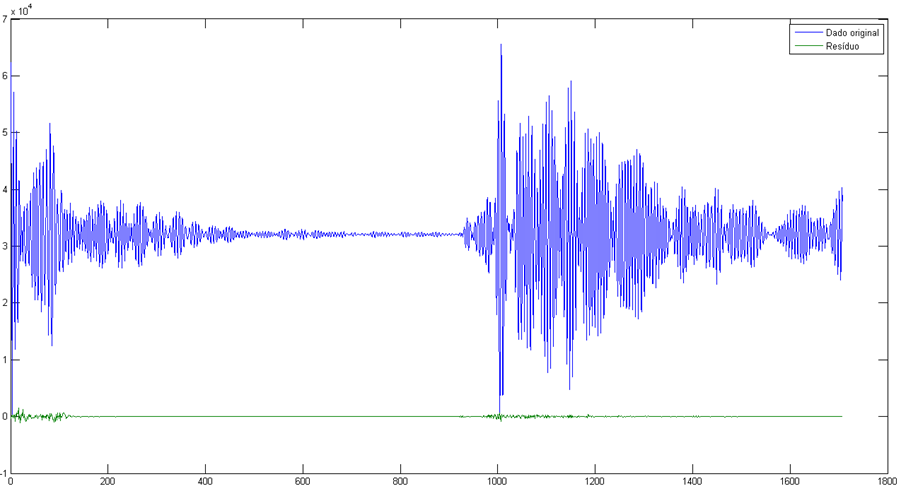
\includegraphics[scale=0.65]{fig/tracoeresiduo.png}
\caption{A linha azul representa um traço sísmico. A linha verde representa o
resíduo calculado a partir desse traço sísmico.}
\label{fig:tracoeresiduo}
\end{figure}

\section{Revisão de trabalhos relacionados}
\label{Sec:trabalhosrelacionados}

Definitivamente, a utilização de predição linear não é novidade na compressão de
dados sísmicos. Movido pela sua ampla utilização, na época, em
processamento de voz,~\citep{Artigo:bordley1983} utilizou a predição linear para a compressão de
dados sísmicos, porém com perdas. Mais tarde, com o
mesmo objetivo,~\citep{Artigo:linearmelhor} mostrou que a predição linear
obteve resultados melhores que as Transformada Discreta de Fourier, Transformada Discreta do Cosseno, Transformada de Walsh-Hadamard e a Tranformada
de Karhunen-Loeve. No trabalho de~\citep{Artigo:stearnsincompleto} são
apresentados, pela primeira vez, o termo~\emph{compressão em duas
etapas}~(\emph{two stage compression}), bem como a
Figura~\ref{Figura:compressaoduasetapas}. Além disso, o autor delimita bem a
importância da predição linear para a decorrelação do dado, e foi pioneiro em
utilizá-la na exata recuperação dele, resultando em uma compressão sem
perdas. Os trabalhos que se seguiram utilizaram a metodologia explicada pelo
autor para comprimir dados sem perdas usando predição linear.  

Um estudo comparativo de compressão de dados sísmicos, sem perdas, foi feito
em~\citep{Artigo:lpemaistres} entre predição linear e outros dois métodos que
se utilizam de diferenciação na primeira etapa, e diferentes algoritmos de
compressão na segunda. Mais uma vez, a predição linear mostrou melhores
resultados na compressão. Em~\citep{Article:twostagecompression}, uma versão
modificada da predição linear, utilizando coeficientes discretos, é apresentada
pelo autor. É possível perceber que os trabalhos acima mudam uma pequena parte
do processo e publicam a novidade. Em~\citep{Artigo:nenhumamudanca}, nenhuma
mudança no processo foi feita, mas os autores citam que conseguiram chegar à
entropia do dado. Em bases teóricas, portanto, não haveria mais meios de
comprimi-lo, assumindo que sua autocorrelação foi totalmente removida. Conforme
a aquisição sísmica foi se tornando mais fidedigna e com maior precisão
numérica, percebeu-se a necessidade de dividir o dado sísmico em subconjuntos.
Como tipicamente dados sísmicos são não-estacionários e previsíveis por apenas
pequenos intervalos. Por isso,~\citep{Artigo:lpjanela} propôs não criar um modelo para todo o dado
sísmico, mas para pequenas janelas nele. Essa abordagem, além de paralelizável, é
computacionalmente mais rápida, porque calcular $N$ modelos com $M$ valores cada
um é computacionalmente menos complexo do que calcular um modelo com $N\times M$ valores.

Em~\citep{Artigo:lpmenosvariancia}, um estudo comparativo entre a predição
linear e outros três métodos utilizando diferenciação foi feito. O trabalho
concluiu que os métodos de diferenciação são computacionalmente menos complexos,
mas geram dados com variância mais elevada, comprometendo o resultado final da
compressão. Já em~\citep{Artigo:lppcm} foi desenvolvido um estudo em que a
predição linear foi comparada a sucessivas diferenças no dado combinada com
Modulação por código de pulsos (PCM), método geralmente usado para representar
digitalmente amostras de sinais analógicos. O resultados foram satisfatórios
para o novo método desenvolvido, já que foram comparáveis aos conseguidos pela
predição linear, mas executaram em um tempo bem inferior.

Como a predição linear pode gerar resíduos não-inteiros, e alguns algoritmos de
compressão não funcionam com esse tipo de dado, foi proposto
em~\citep{Artigo:stearn} uma forma de contornar esse problema, bem como de
diminuir o número de símbolos gerados pela predição linear. Tal solução será
utilizada nesse trabalho e, por esse motivo, já foi explicada na
Seção~\ref{Paragrafo:stearns}. Em~\citep{Artigo:lpearma}, o modelo ARMA foi
utilizado para a compressão de dados sísmicos sem perda. A abordagem foi
comparada aos modelos autoregressivo e de diferenciação. O resultado, de acordo
com os autores, foi excelente, pois foi superior ao método de diferenciação e
comparável ao método de predição linear.

Conforme citado na Seção~\ref{Paragrafo:bemcalculado}, um modelo bem
calculado é aquele que consegue um conjunto de resíduos minizado. Existem alguns
algoritmos com esse propósito, e foi justamente o desempenho de alguns
desses algoritmos que~\citep{Artigo:lpcomparacao} comparou. Portanto, seu
trabalho evidenciou que a própria predição linear pode apresentar resultados
melhores, se o algoritmo mais propício for escolhido. O cálculo dos parâmetros
da predição linear requer tempo e, por isso, sua utilização para compressão em
tempo real se torna difícil. Sob essa ideia, outra comparação entre o modelo de
predição linear e diferenciação foi feita
em~\citep{Artigo:lpediferenciacaodenovo} com os mesmos resultados obtidos
em~\citep{Artigo:lpmenosvariancia}, ou seja, é comparável à predição linear,
mas computacionalmente menos complexa. Ainda na onda de
comparações, em~\citep{Artigo:lparmadenovo} e~\citep{Artigo:lparmadenovo2}, a
predição linear foi novamente comparada ao modelo ARMA, e os resultados foram bem semelhantes. A métrica
utilizada foi a divisão do tamanho comprimido pelo original do dado, e a
diferença obtida entre os modelos ocorreu na segunda casa decimal em todos os
experimentos e em ambos os trabalhos.

Em~\citep{Artigo:naolinearestat}, é proposto um método de compressão de dados
sísmicos sofisticado, pelas palavras do autor. Utilizando algum mistério, o
artigo limita-se a dizer que utilizou uma transformada associada a um método
estatístico não-linear, embora não tenha especificado qual.

Como citado na Seção~\ref{Paragrafo:descorrelacaoprimeiraetapa}, o objetivo
da primeira etapa no processo de compressão de dados é a decorrelação e
diminuição da variância do dado original. Eventualmente, um modelo pode não ser
capaz de remover toda a autocorrelação do dado, apenas reduzi-la. Pensando
nisso,~\citep{Artigo:multiplepasses} propõe passar o dado original pelo modelo
de predição linear e, caso o resíduo gerado não seja totalmente decorrelacionado,
passar o resíduo calculado novamente pelo modelo, repetindo esse processo até se
obter o resultado desejado. O trabalho reporta que a compressão foi melhorada
notavelmente através desse processo.

Em~\citep{Artigo:lpparalelizado}, uma estratégia de paralelização do modelo de
predição linear utilizando redes de sensores sem fio é desenvolvida. Um dos
grandes méritos do trabalho é permitir compressão dos dados em tempo real, algo
até então só conseguido com o método de diferenciação. Também utilizando
sensores sem fio,~\citep{Artigo:lpsemfio} utiliza predição linear para comprimir
dados sísmicos de monitoramento de certos campos, como vulcões. Tais trabalhos
são interessantes porque, além de mostrarem a faceta parelelizável da predição
linear, também precisam se preocupar com diversos fatores limitadores presentes
nas redes de sensores sem fio, como perda de pacotes de dados e baixo poder
computacional. Em um dos trabalhos mais recentes de compressão de dados
sísmicos,~\citep{Artigo:pcalinenaolin} estuda o método de análise de
componentes principais não-linear combinado com redes neurais
auto-associativas para este fim. Sem entrar em muitos detalhes nos resultados
obtidos, mas no método em si, o artigo aponta que o método proposto pode ser
utilizado na compressão de dados sísmicos sem perdas com êxito.

Saindo um pouco do escopo de modelos preditivos, como o AR e o ARMA, é possível
descorrelacionar o dado sísmico através de transformadas. Essa estratégia de
compressão também é bem aceita. Alguns métodos utilizados são 
a transformada discreta de Fourier, a transformada discreta do cosseno, a
transformada de Walsh-Hadamard e a transformada de Karhunen-Loeve.
Em~\citep{Artigo:comparartransformadas} tais transformadas foram comparadas, com
atenção especial à transformada discreta do cosseno, que foi capaz de reduzir o
tamanho do dado original em um terço, sem perdas. Mais
tarde,~\citep{Artigo:dctruim} reportou que a transformada discreta do cosseno
adiciona artefatos indesejáveis ao dado comprimido. A compressão, portanto, não
pode ser considerada sem perdas, pois o dado original não é reconstruído com
exatidão.

Atualmente, os trabalhos de compressão de dados sísmicos sem perdas focam na
utilização de abordagens paralelas utilizando rede de sensores sem fio e GPU.
Em~\citep{Artigo:transformadainteiro} foi proposta uma forma de paralelizar
Transformada Inteira de Gram-Schmidt para redes de sensores sem fio. Tal
plataforma também foi utilizada por~\citep{Artigo:volcano} para monitoramento de
atividades sísmicas em vulcões. Em GPUs, um trabalho que se destaca foi o
proposto em~\citep{Artigo:gpurealtime}, em que o autor relata uma
solução de compressão em tempo real utilizando GPUs através de manipulação e
compressão direta de sequências de bits.

Por certo, os modelos AR e ARMA são bem vistos no cenário de compressão de
dados. Entretanto, apesar de seus bons resultados, tais modelos são lineares,
diferente do dado sísmico que é heteroscedástico. Apesar de conseguirem, os
modelos AR e ARMA demoram mais iterações para convergir nesse cenário, pois não
estão preparados para as súbitas mudanças nos valores dos dados. Embora alguns
trabalhos já tenham utilizados modelos não-lineares para calcular os parâmetros
do dado sísmico, não fomos capazes de encontrar algum que lide diretamente com
sua heteroscedasticidade.

\section{Método de compressão utilizando ARIMA-GARCH}

A Equação~\ref{Equacao:razaocompressao} apresenta a métrica a ser utilizada
nesse trabalho.

\begin{equation}
\text{Razão compressão} = \frac{\text{Tamanho Original}}{\text{Tamanho
comprimido}}
\label{Equacao:razaocompressao}
\end{equation}

% \begin{algorithm}
% \caption{Algoritmo de testes}
% \label{algo:explicacao}
% idade $\leftarrow$ 0\;
% responsabilidade $\leftarrow$ 0\;
% \Enqto{idade $<$ 100}{
% 	\Enqto{responsabilidade $<$ 10}{
% 		\tcp{Inicia contador}
% 		\tcp{Rodar sistema nebuloso}
% 		\tcp{Para contador}
% 		responsabilidade $\leftarrow$ responsabilidade + 0.1\;
% 	}
% 	idade $\leftarrow$ idade + 0.5\;
% }
% \end{algorithm}

% Stochastic ARIMA-GARCH Entropy Encoding for Seismic Data 


 \begin{algorithm}
\caption{O algoritmo de compressão}
\label{Algoritmo:SAGE}
\Entrada
{
\begin{description}
  \item[dado\_original]\\
  	Vetor coluna contendo os valores sísmicos a serem comprimidos
  \item[num\_bits]\\
  	Número inteiro indicando a precisão numérica dos dados a serem comprimidos.
  	Esse parâmetro é importante para quantizar o número para uma representação inteira.
  \item[num\_bin]\\
  	Número inteiro indicando o quociente a ser utilizado no algoritmo de Stearns.
  \item[n\_ar]\\
  	Número inteiro indicando o parâmetro autoregressivo do modelo ARIMA-GARCH.
  \item[n\_ma]\\
  	Número inteiro indicando o parâmetro de médias móveis do modelo ARIMA-GARCH.
  \item[n\_d]\\
  	Número inteiro indicando o parâmetro de diferenças do modelo ARIMA-GARCH.
  \item[n\_arch]\\
  	Número inteiro indicando o parâmetro ARCH do modelo ARIMA-GARCH.
  \item[n\_garch]\\
  	Número inteiro indicando o parâmetro GARCH do modelo ARIMA-GARCH.
\end{description}
}
\Saida
{
\begin{description}
  \item[pacote\_compressao]\\
  	Um objeto contendo todos os dados necessários para a descompressão do dado
  	sísmico.
\end{description}
}
\Inicio
{

% \tcc{Primeiro passo. Preparando o dado. Nessa etapa o dado é passado da sua
% representação em ponto flutuante para uma representação em números inteiros, sem
% perda de suas características estatísticas. Nesse algoritmo, essa transformação
% é feita pela função uencode, que recebe como primeiro argumento o dado a ser
% quantizado e o segundo a precisão numérica do dado.}
dado\_quantizado \rec quantiza\_para\_inteiro(dado\_original,
num\_bits) \; modelo \rec new Arima(n\_ar, n\_ma, n\_d)\;
\Se{n\_arch $\neq$ 0 \textbf{Ou} n\_garch $\neq$ 0}
{
modelo.Variance \rec new Garch(n\_arch, n\_garch)\;
}

modelo.Estimar(dado\_quantizado)\;
\eSe{modelo.Convergiu}
{
	residuo \rec modelo.Calcular\_Residuo(dado\_quantizado)\;
}
{
	residuo \rec dado\_quantizado\;
	modelo \rec null\;
}
[$A_O$, $A_B$] \rec Algoritmo\_Stearns(residuo) \;
res\_comp \rec Codificacao\_Aritmetica($A_B$)\;
pacote\_compressao \rec Monta\_Pacote\_Comp(modelo, residuo)\;
\Retorna pacote\_compressao\;
}
\end{algorithm}

O Algoritmo~\ref{Algoritmo:SAGE} ilustra a solução proposta neste trabalho mais
a fundo. Na linha 2, o algoritmo chama a função quantiza\_para\_inteiro. O objetivo dessa função
é quantizar os dados para uma representação numérica inteira, ao invés de ponto
flutuante, sem perder as características estatísticas do dado. Faz-se isso para
evitar problemas de precisão numérica que poderiam comprometer a característica do algoritmo ser sem perdas. A função quantiza\_para\_inteiro
precisa dos dados normalizados no intervalo $[-1, +1]$, bem como a precisão, em
bits, dos dados. O algoritmo~\ref{Algoritmo:SAGE} não demonstra a etapa de
normalização dos dados porque ela foge do escopo desse trabalho.

A linha 3 do algoritmo indica a criação de um objeto do tipo ARIMA. No seu
construtor, são passados o parâmetro autoregressivo, o de média móveis e o
número de diferenças a serem calculadas pelo modelo. A linha 4 decide se devemos
utilizar um modelo puramente ARIMA ou se desejamos incluir o GARCH formando o
modelo ARIMA-GARCH. Tal decisão é feita de acordo com o parâmetro ARCH e GARCH
informados. A linha 5 inicia a variância do modelo ARIMA utilizando GARCH, com
seus respectivos parâmetros.

Na linha 7 a estimativa dos parâmetros do modelo é iniciada. Repare que foi
informado o parâmetro dado\_quantizado para o método, não dado\_original. A
linha 8 verifica se o modelo conseguiu convergir. Caso positivo, a linha 9 é
executada, a fim de calcular o resíduo (diferença entre o dado real e o
calculado pelo modelo). Caso negativo, a linha 11 é executada, e o dado
comprimido é o próprio dado\_quantizado, sem a utilização do ARIMA-GARCH.

A linha 13 chama o algoritmo de Steans (Seção~\ref{Paragrafo:stearns}),
retornando duas séries numéricas a partir do resíduo calculado, $A_O$ e $A_B$.
$A_B$ é comprimido na linha 14 usando a codificação aritmética. A linha 15
ilustra a criação do pacote de compressão. Esse pacote será enviado ao
decodificador para que o dado original seja obtido. O decodificador assume que
se o modelo informado for nulo, significa que a solução não convergiu. Caso
contrário, todos os valores dos parâmetros do ARIMA-GARCH estão no objeto
modelo.

A implementação desse trabalho foi realizada no software MatLab versão 2013a. Os
testes foram rodados em um Core i7 2630QM (2.0 GHz), 8GB de memória RAM, Windows
8.1 64 bits.
